\documentclass{lab_sheet}
\usepackage{hyperref}
\usepackage{longtable}
\usepackage{alltt}
\def\ddfrac#1#2{\displaystyle\frac{\displaystyle #1}{\displaystyle #2}}
\begin{document}
\titlePage{Design of IIR Digital Filters}{January 23, 2022}
\pagenumbering{roman}
\clearpage
\tableofcontents
\clearpage
\phantomsection
\addcontentsline{toc}{section}{\bfseries{List of Figures}}
\listoffigures
\clearpage
\phantomsection
\addcontentsline{toc}{section}{\bfseries{Listings}}
\lstlistoflistings
\clearpage
\pagenumbering{arabic}
\section{Objectives}
\begin{itemize}
	\item Familiarization with design of IIR digital filters from analog filter.
	\item Comparison of response for different filter approximations like butterworth, chebyshev I, chebyshev II and elliptic filters.
\end{itemize}
\section{Background Theory}
There are several methods that can be used to design digital filters having an infinite duration unit sample response. One of the popular methods is based on converting an analog filter into a digital filter. In this method we begin the design of digital filter in the analog domain and then convert the design into the digital domain. For this purpose, depending on the specifications of the required digital filter the various approximations like butterworth, chebyshev I, chebyshev II and elliptic filters are used.\\
Among the different approaches used in the design of digital IIR filters this lab experiment deals with impulse invariance method and bi-linear transformation.
\subsection{Impulse Invariance Method}
In impulse invariance method, the objective is to design an IIR filter having an unit sample response $h[n]$ that is the sampled version of the impulse response of the analog filter.
\begin{equation*}
    h[n]=h[nT] \quad \quad n=0,1,2,\dots\dots, \text{where } T\text{ is the sampling interval}
\end{equation*}
\subsection{Bi-Linear Transformation}
In bi-linear transformation a conformal mapping from s-plane to z-plane is carried out with the relation given as,
\begin{equation*}
    s=\frac{2}{T}\left(\frac{1-z^{-1}}{1+z^{-1}}\right)
\end{equation*}
\section{Functions Used}
\begin{longtable}[H]
    {|l||m{0.5\linewidth}|}
        \hline
        \textbf{Function with syntax}&\textbf{Description}\\
        \hline\hline
        \texttt{[bz,az]=impinvar(b,a,fs)}&Creates a digital filter with coefficients bz and az, whose impulse response is equal to the impulse response of the analog filter with coefficients b and a, scaled by $1/f_s$, where $f_s$ is the sample rate.\\
        \hline
        \texttt{[numd,dend]=bilinear(num,den,fs)}&Converts the s-domain transfer function specified by coefficients num and den to a discrete equivalent.\\
        \hline
        \texttt{[n,Wc]=buttord(Wp,Ws,Rp,Rs)}
        &Returns the lowest order n of the butterworth filter and scalar (or vector) of corresponding cutoff frequencies Wc. \\
        \hline
        \texttt{[n,Wp]=cheb1ord(Wp,Ws,Rp,Rs)}
        &Returns the lowest order n of the chebyshev I filter and scalar (or vector) of corresponding cutoff frequencies Wp. \\
        \hline
        \texttt{[n,Ws]=cheb2ord(Wp,Ws,Rp,Rs)}
        &Returns the lowest order n of the chebyshev II filter and scalar (or vector) of corresponding cutoff frequencies Ws. \\
        \hline
        \texttt{[n,Wp]=ellipord(Wp,Ws,Rp,Rs)}
        &Returns the lowest order n of the elliptic filter and scalar (or vector) of corresponding cutoff frequencies Wc.\\
        \hline
        \texttt{[b,a]=butter(n,Wc)}&Returns the transfer function coefficients of an nth-order lowpass digital butterworth filter with normalized cutoff frequency Wc.\\
        \hline
        \texttt{[b,a]=cheby1(n,Rp,Wp)}&Returns the transfer function coefficients of an nth-order lowpass digital chebyshev I filter with normalized pass band edge frequency Wp and Rp decibels of peak-to-peak pass band ripple.\\
        \hline
        \texttt{[b,a]=cheby2(n,Rs,Wp)}&Returns the transfer function coefficients of an nth-order lowpass digital chebyshev II filter with normalized stop band edge frequency Ws and Rs decibels of stop band attenuation down from the peak pass band value.\\
        \hline
        \texttt{[b,a]=ellip(n,Rp,Rs,Wp)}&Returns the transfer function coefficients of an nth-order lowpass digital elliptic filter with normalized pass band edge frequency Wp. The resulting filter has Rp decibels of peak-to-peak pass band ripple and Rs decibels of stop band attenuation down from the peak pass band value.\\
        \hline
        \texttt{impulse(b, a, Tfinal)}&Plots the impulse response of system with coefficients b and a  from t = 0 to the final time t = Tfinal.\\
        \hline
        \texttt{dimpulse(bz, az)}&Plots the impulse response of system with coefficients bz and az.
        \\
        \hline
\end{longtable}
\section{Lab Exercises}
\mysub{Conversion of analog to digital filter}
\problem{a. Convert the analog filter $H_a(s)=\ddfrac{s+0.1}{(s+0.1)^2+9}$ into a digital IIR filter by means of the
impulse invariance method. Plot the frequency response (magnitude) of the designed filter taking sampling interval $(T)$ of 0.1, 0.5 seconds. Compare the response of the filter designed to that of the analog one. Comment on the effect of $T$ on the response.}
\subproblem{b. Compare the unit sample response of the designed digital IIR filter with the impulse response
of analog filter for $T$=0.1 and 0.5.}
\subproblem{c. Convert the above analog filter in to a digital IIR filter by means of bilinear transformation
and repeat all the procedures as specified in Problem 1.a.}
\matlabcode{transformation_selector}{Matlab function to convert analog to digital IIR filter using user selection and plot impulse response }
\matlabcode{lab_5_a}{Matlab script to plot magnitude response comparison for analog and digital filter}
\mysubsub{Using impulse invariance method}
\begin{figure}[H]
    \centering
    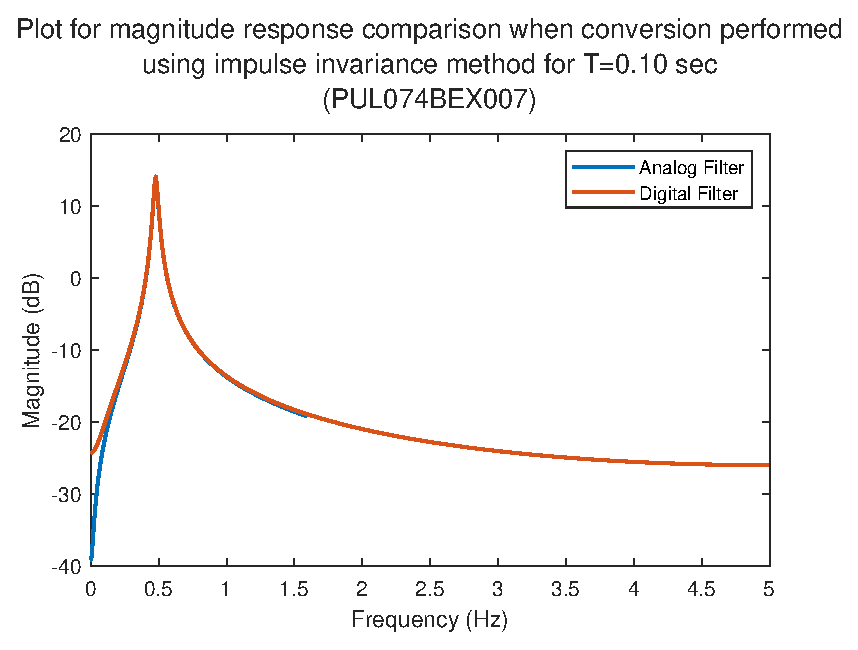
\includegraphics[width=0.7\linewidth]{../Figures/mag_res_impulse invariance method_0.eps}
    \caption{Plot for magnitude response comparison when conversion performed with impinvar and $T=0.1$ second}
    \label{fig:5_1_a}
\end{figure}

\begin{figure}[H]
    \centering
    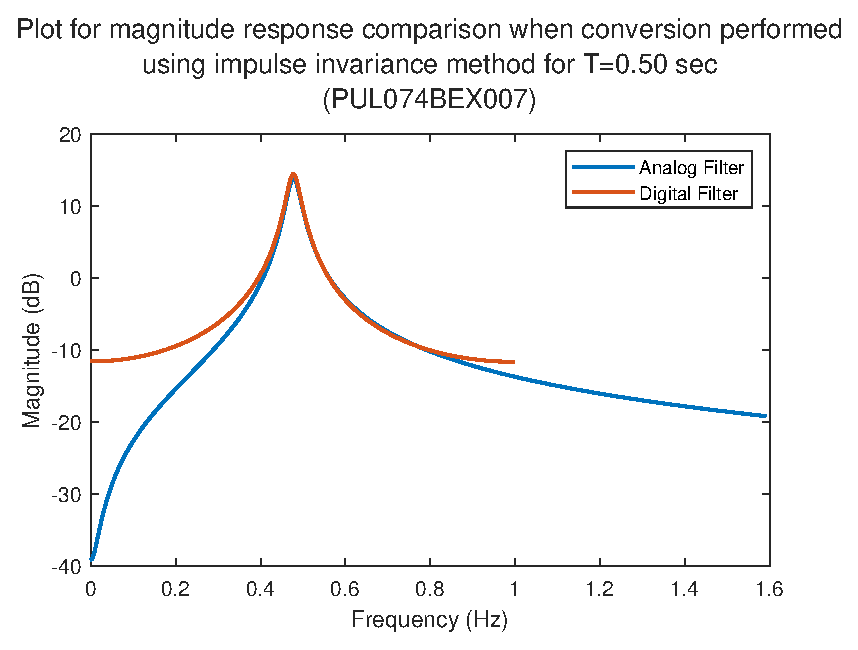
\includegraphics[width=0.7\linewidth]{../Figures/mag_res_impulse invariance method_1.eps}
    \caption{Plot for magnitude response comparison when conversion performed with impinvar and $T=0.5$ second}
    \label{fig:5_1_b}
\end{figure}

\begin{figure}[H]
    \centering
    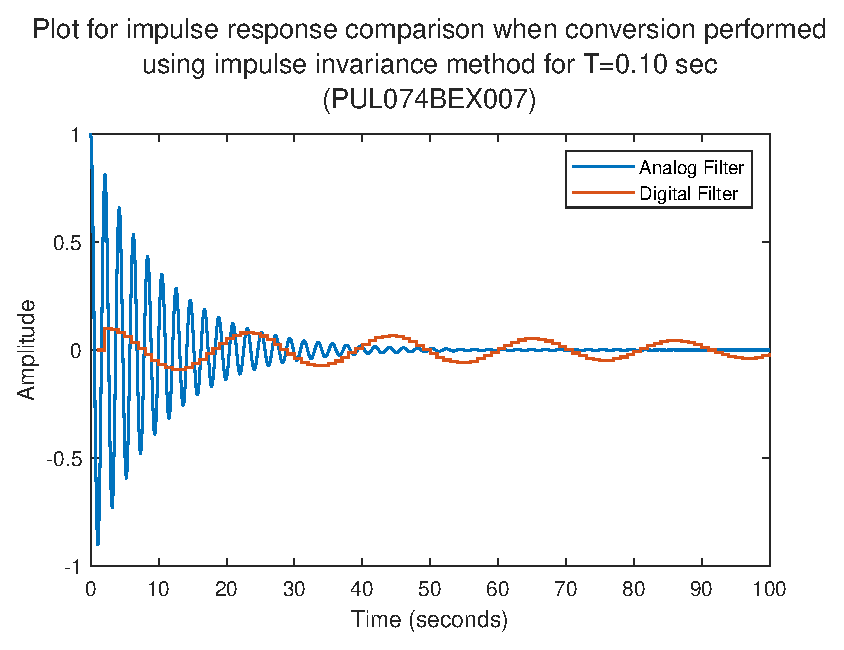
\includegraphics[width=0.7\linewidth]{../Figures/impulse_res_impulse invariance method_0.eps}
    \caption{Plot for impulse response comparison when conversion performed with impinvar and $T=0.1$ second}
    \label{fig:5_1_c}
\end{figure}

\begin{figure}[H]
    \centering
    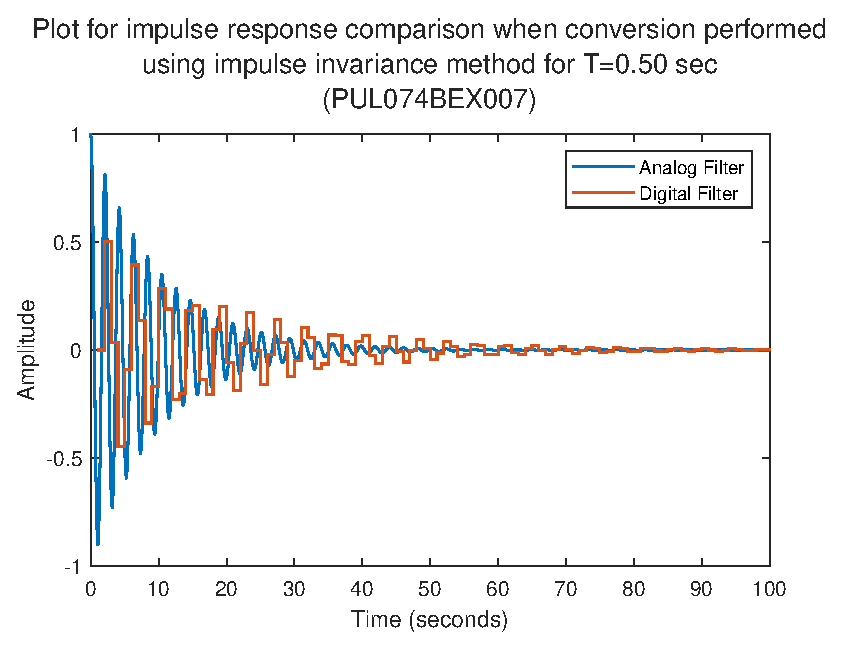
\includegraphics[width=0.7\linewidth]{../Figures/impulse_res_impulse invariance method_1.eps}
    \caption{Plot for impulse response comparison when conversion performed with impinvar and $T=0.5$ second}
    \label{fig:5_1_d}
\end{figure}

\mysubsub{Using bilinear transformation}
\begin{figure}[H]
    \centering
    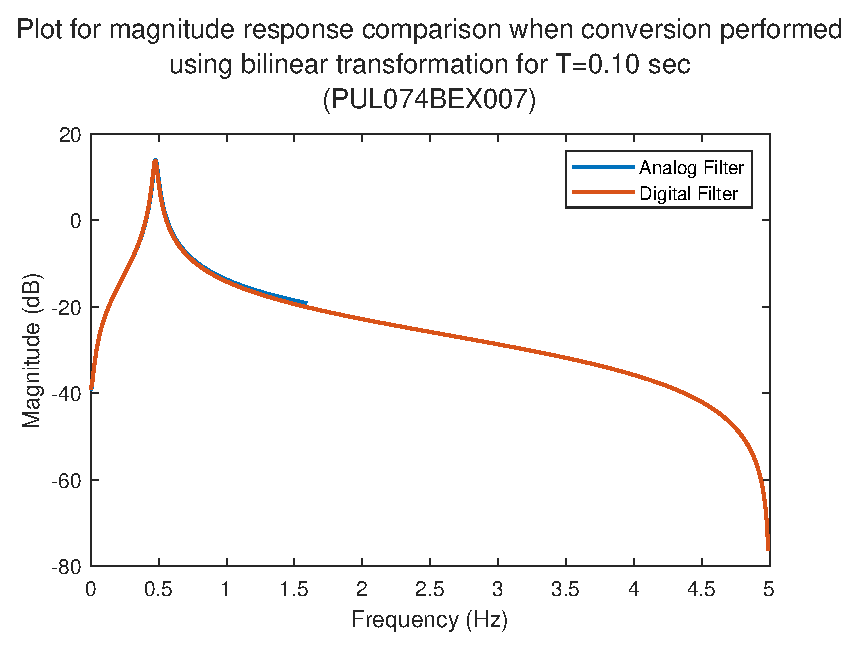
\includegraphics[width=0.7\linewidth]{../Figures/mag_res_bilinear transformation_0.eps}
    \caption{Plot for magnitude response comparison when conversion performed with bilinear and $T=0.1$ second}
    \label{fig:5_1_e}
\end{figure}

\begin{figure}[H]
    \centering
    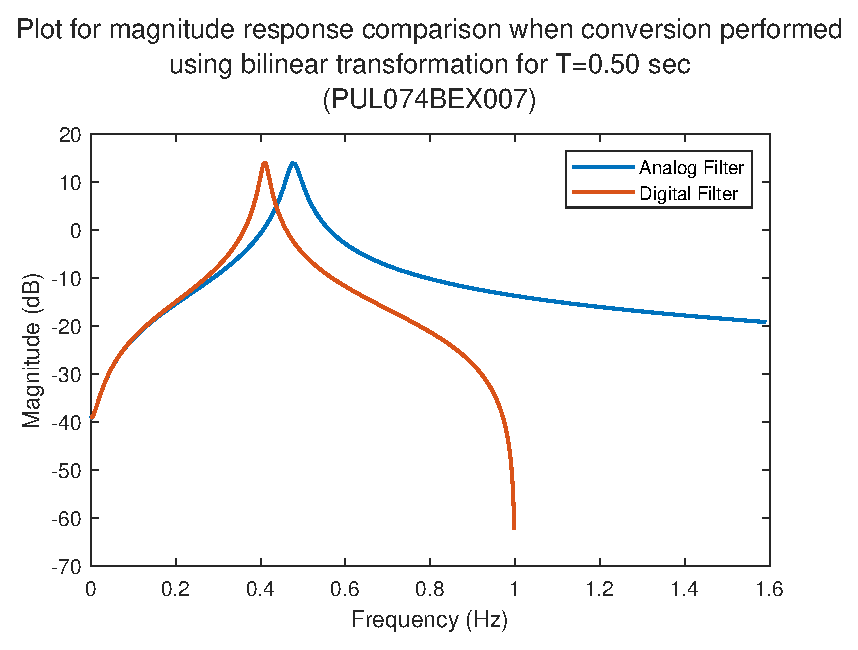
\includegraphics[width=0.7\linewidth]{../Figures/mag_res_bilinear transformation_1.eps}
    \caption{Plot for magnitude response comparison when conversion performed with bilinear and $T=0.5$ second}
    \label{fig:5_1_f}
\end{figure}

\begin{figure}[H]
    \centering
    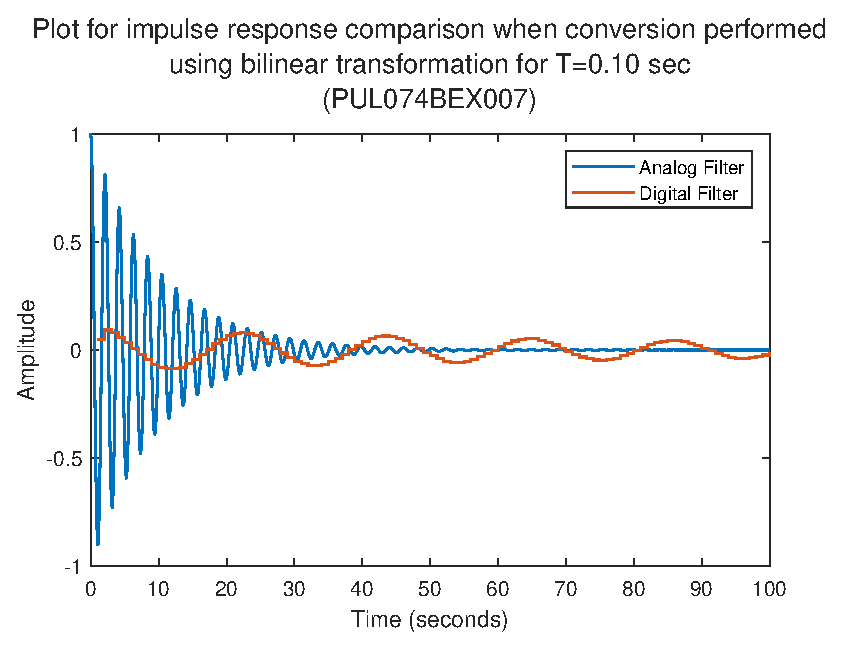
\includegraphics[width=0.7\linewidth]{../Figures/impulse_res_bilinear transformation_0.eps}
    \caption{Plot for impulse response comparison when conversion performed with bilinear and $T=0.1$ second}
    \label{fig:5_1_g}
\end{figure}

\begin{figure}[H]
    \centering
    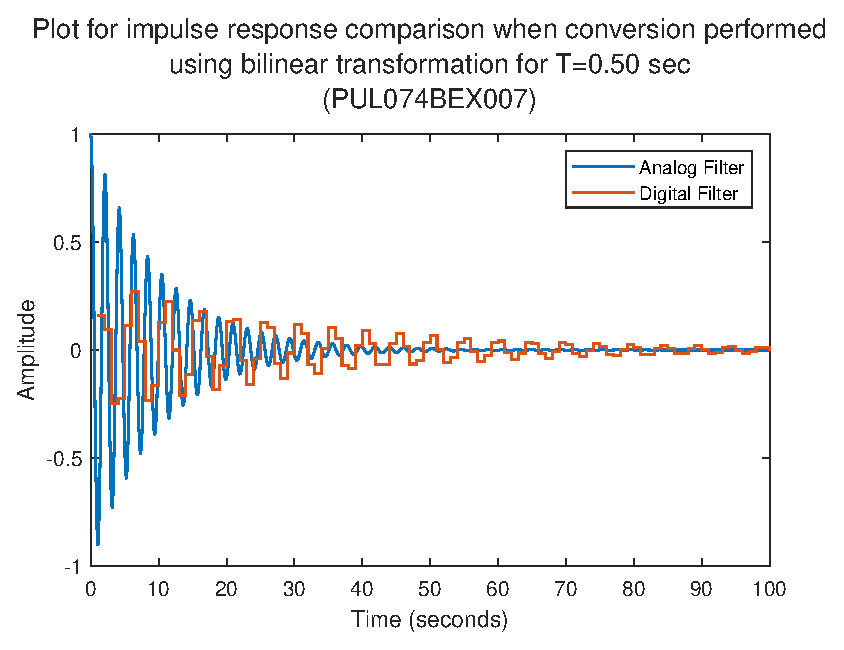
\includegraphics[width=0.7\linewidth]{../Figures/impulse_res_bilinear transformation_1.eps}
    \caption{Plot for impulse response comparison when conversion performed with bilinear and $T=0.5$ second}
    \label{fig:5_1_h}
\end{figure}
\mysubsub{Comparison between the two methods}
From the observations in Figure~\ref{fig:5_1_a} and Figure~\ref{fig:5_1_b} it is visible that the converted digital filter has somewhat of a similar magnitude response when compared with analog filter. However, the digital filter undergoes spectrum aliasing. This is due to the fact that s-plane to z-plane mapping is many-to-one, i.e., all poles in s-plane between $\left[\ddfrac{(2k-1)\pi}{T},\ddfrac{(2k+1)\pi}{T}\right]$ where $k=0,1,2,\dots\dots$ map into the entire z-plane, which leads to infinite number of poles mapped onto the same location thus producing aliasing effect. Due to this fact the impulse invariance method is not preferred while designing IIR filter other than lowpass nature. When the sampling time $(T)$ is increased it generally results in a frequency response that is more spaces out hence decreasing the chances of aliasing. However, this is not the case with impulse invariance method. Hence the increase in sampling time has no effect on the reduction of aliasing that happens. \\
Similarly, from the observations in Figure~\ref{fig:5_1_e} and Figure~\ref{fig:5_1_f}, there is no visible aliasing effect. This is due to the fact that s-plane to z-plane mapping is one-to-one. Due to this fact the bilinear transformation has no restriction on the type of filter that can be transformed. The only known disadvantage of the bilinear transformation is the frequency warping, which is the effect where there exists a non-linear relationship between the continuous time filter frequency and discrete time filter frequency. To compensate for this phenomena, a technique called pre-warping is applied.
\mysub{Design of IIR digital lowpass filter for given specifications}
\problem{An IIR digital low pass filter is required to meet the following specifications:}
\begin{alltt}
    Pass band ripple (or peak to peak ripple):\ensuremath{\leq} 0.5 dB
    Pass band edge: 1.2 kHz
    Stop band attenuation:\ensuremath{\geq} 40 dB
    Stop band edge: 2.0 kHz
    Sample rate: 8.0 kHz
\end{alltt}
\textbf{Use the MATLAB Signal Processing Toolbox functions to determine, the required filterorder, the cutoff frequency, the numerator and the denominator coefficients for the dig­ital Butterworth, digital Chebyshev and digital Elliptic filters. Also plot their frequency responses. Describe the nature of each response.}
\matlabcode{filter_selector}{Matlab function to select particular filter type based on user input}
\matlabcode{lab_5_b}{Matlab script to plot frequency response, display cutoff frequency and order of selected filter}
\pagebreak
\mysubsub{Butterworth approximation}
\begin{verbatim}
    >>lab_5_b         
    Enter the filter type: butterworth
    Order of butterworth filter=9
\end{verbatim}
\begin{figure}[H]
    \centering
    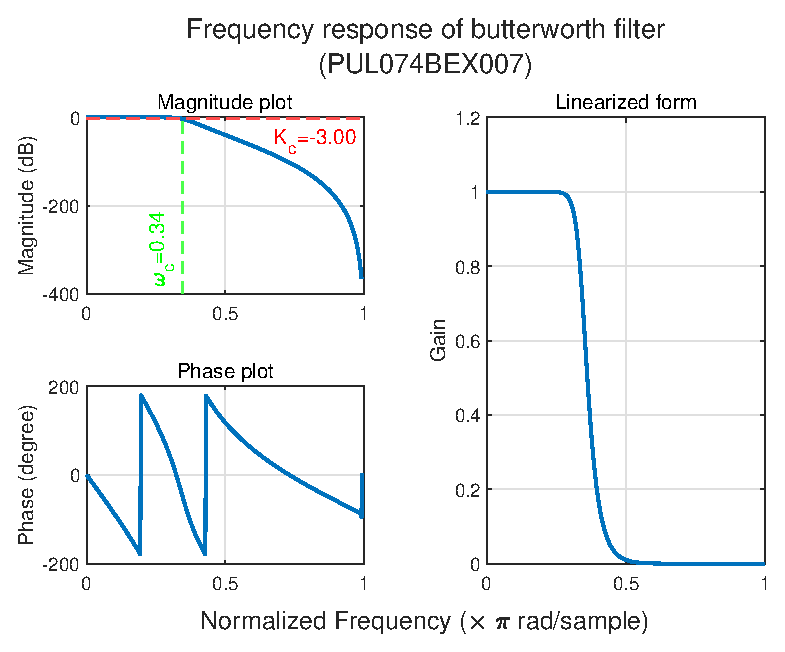
\includegraphics[width=0.9\linewidth]{../Figures/butterworth.eps}
    \caption{Plot for frequency response of butterworth filter}
    \label{fig:5_2_butter}
\end{figure}
From the observations in Figure~\ref{fig:5_2_butter}, the nature of the filter is lowpass. There is no ripple in the passband or the stopband of the filter, i.e. it is maximally flat. The cut-off frequency is 0.34 ($\times \pi$ rad/sample), which coincides with the plot at $-3$ dB. The order of the filter is 9.  
\pagebreak
\mysubsub{Chebyshev I approximation}
\begin{verbatim}
    >> lab_5_b
    Enter the filter type: chebyshev I
    Order of chebyshev I filter=5
\end{verbatim}
\begin{figure}[H]
    \centering
    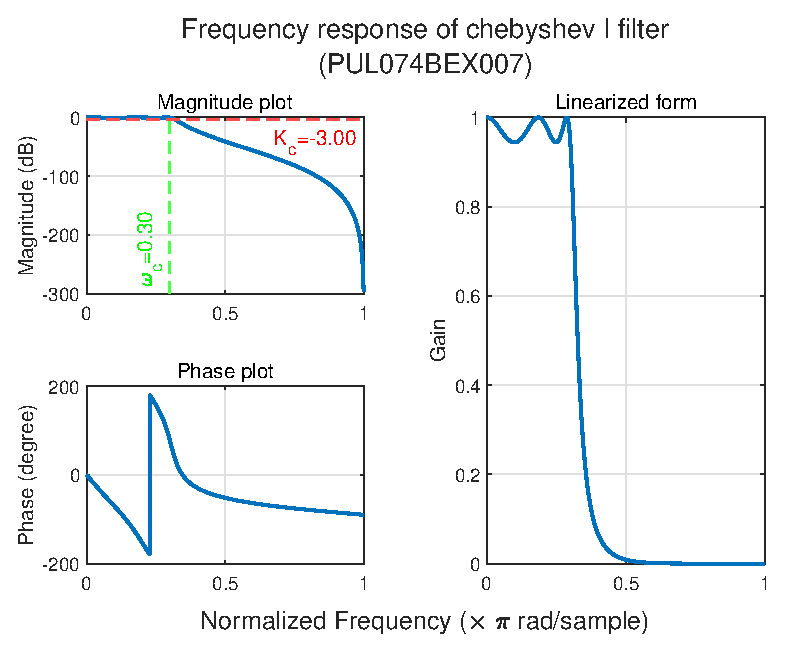
\includegraphics[width=0.9\linewidth]{../Figures/chebyshev I.eps}
    \caption{Plot for frequency response of chebyshev I filter}
    \label{fig:5_2_cheby1}
\end{figure}
From the observations in Figure~\ref{fig:5_2_cheby1}, the nature of the filter is lowpass. There is visible ripple in the passband but no ripple is seen in the stopband of the filter. The passband ripple is $\leq0.5$ dB. The cut-off frequency is 0.30 ($\times \pi$ rad/sample), which is actually the passband edge in normalized form. The order of the filter is 5.  
\pagebreak
\mysubsub{Chebyshev II approximation}
\begin{verbatim}
    >> lab_5_b
    Enter the filter type: chebyshev II
    Order of chebyshev II filter=5
\end{verbatim}
\begin{figure}[H]
    \centering
    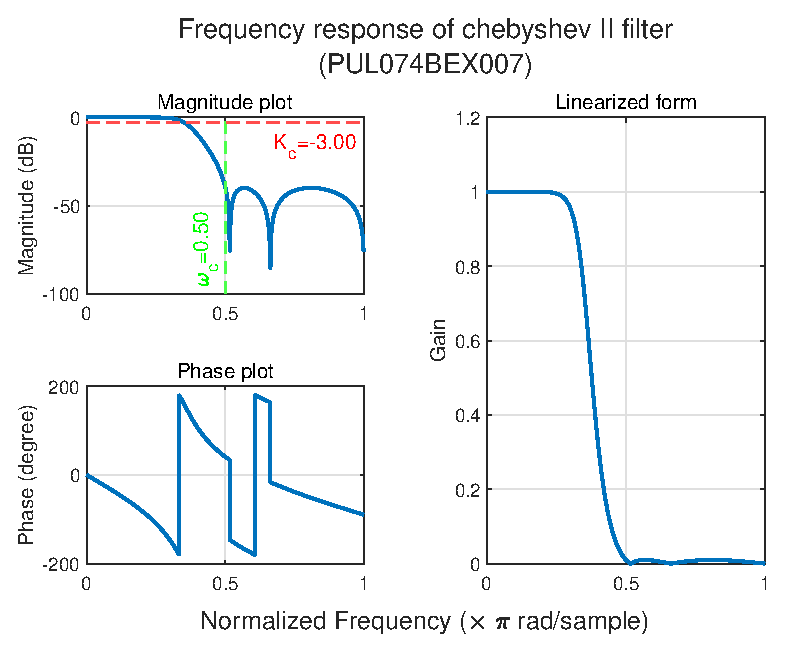
\includegraphics[width=0.9\linewidth]{../Figures/chebyshev II.eps}
    \caption{Plot for frequency response of chebyshev II filter}
    \label{fig:5_2_cheby2}
\end{figure}
From the observations in Figure~\ref{fig:5_2_cheby2}, the nature of the filter is lowpass. There is visible ripple in the stopband but no ripple is seen in the passband of the filter. The stopband attenuation is $\geq40$ dB. The cut-off frequency is 0.50 ($\times \pi$ rad/sample), which is actually the stopband edge in normalized form. The order of the filter is 5. 
\pagebreak
\mysubsub{Elliptic approximation}
\begin{verbatim}
    >> lab_5_b
    Enter the filter type: elliptic
    Order of elliptic filter=4
\end{verbatim}
\begin{figure}[H]
    \centering
    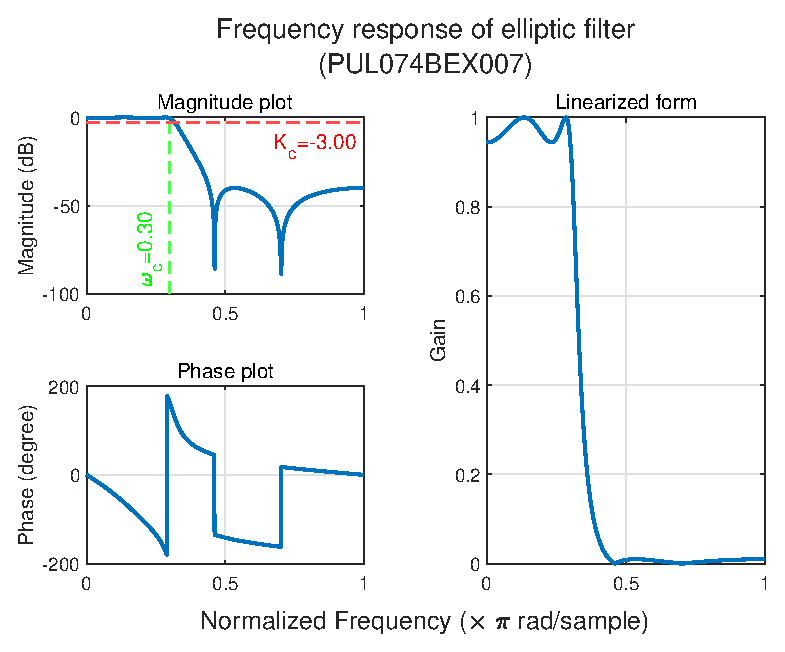
\includegraphics[width=0.9\linewidth]{../Figures/elliptic.eps}
    \caption{Plot for frequency response of elliptic filter}
    \label{fig:5_2_ellip}
\end{figure}
From the observations in Figure~\ref{fig:5_2_ellip}, the nature of the filter is lowpass. There is visible ripple in both the passband and the stopband of the filter. The passband ripple is $\leq0.5$ dB and the stopband attenuation is $\geq40$ dB. The cut-off frequency is 0.30 ($\times \pi$ rad/sample), which is actually the passband edge in normalized form. The order of the filter is 4. 
\mysubsub{Comparison between the filter types}
\begin{table}[H]
    \centering
    \begin{tabular}{|m{0.3\linewidth}||m{0.2\linewidth}||m{0.2\linewidth}||m{0.1\linewidth}|}
        \hline
        \textbf{Filter Type}&\textbf{Passband}&\textbf{Stopband}&\textbf{Order}\\\hline\hline
        Butterworth&Flat&Flat&9\\\hline
        Chebyshev I&Equiripple&Flat&5\\\hline
        Chebyshev II&Flat&Equiripple&5\\\hline
        Elliptic&Equiripple&Equiripple&4\\\hline
    \end{tabular}
\end{table}
From the summarized comparison, it is clear that there is a tradeoff between monotonic response and the order of the filter. For the maximally flat butterworth filter, the order is 9, which on contrast is 4 for the elliptic filter which has equiripple in both the passband and the stopband.
\section{Discussion and Conclusion}
In this lab experiment we dealt with the design of IIR filters. Firstly, conversion of analog filters using two methods, viz. impulse invariance method and bilinear transformation was performed. During this, the aliasing effect was noted for impulse invariance method which is why it should not be preferred for designing IIR filter other than lowpass nature. However, for bilinear transformation such effect wasn't seen, so it has no restriction on the type of filter that can be designed. Similarly, the other problem dealt with designing and comparing filter approximation techniques for given IIR digital lowpass specifications. The comparison showed that there is a tradeoff between the monotonic nature and order of filter. \\
Hence, the objectives of the lab experiment were fulfilled.
\end{document}
